% Options for packages loaded elsewhere
% Options for packages loaded elsewhere
\PassOptionsToPackage{unicode}{hyperref}
\PassOptionsToPackage{hyphens}{url}
\PassOptionsToPackage{dvipsnames,svgnames,x11names}{xcolor}
%
\documentclass[
  authoryear,
  preprint]{elsarticle}
\usepackage{xcolor}
\usepackage{amsmath,amssymb}
\setcounter{secnumdepth}{5}
\usepackage{iftex}
\ifPDFTeX
  \usepackage[T1]{fontenc}
  \usepackage[utf8]{inputenc}
  \usepackage{textcomp} % provide euro and other symbols
\else % if luatex or xetex
  \usepackage{unicode-math} % this also loads fontspec
  \defaultfontfeatures{Scale=MatchLowercase}
  \defaultfontfeatures[\rmfamily]{Ligatures=TeX,Scale=1}
\fi
\usepackage{lmodern}
\ifPDFTeX\else
  % xetex/luatex font selection
\fi
% Use upquote if available, for straight quotes in verbatim environments
\IfFileExists{upquote.sty}{\usepackage{upquote}}{}
\IfFileExists{microtype.sty}{% use microtype if available
  \usepackage[]{microtype}
  \UseMicrotypeSet[protrusion]{basicmath} % disable protrusion for tt fonts
}{}
\makeatletter
\@ifundefined{KOMAClassName}{% if non-KOMA class
  \IfFileExists{parskip.sty}{%
    \usepackage{parskip}
  }{% else
    \setlength{\parindent}{0pt}
    \setlength{\parskip}{6pt plus 2pt minus 1pt}}
}{% if KOMA class
  \KOMAoptions{parskip=half}}
\makeatother
% Make \paragraph and \subparagraph free-standing
\makeatletter
\ifx\paragraph\undefined\else
  \let\oldparagraph\paragraph
  \renewcommand{\paragraph}{
    \@ifstar
      \xxxParagraphStar
      \xxxParagraphNoStar
  }
  \newcommand{\xxxParagraphStar}[1]{\oldparagraph*{#1}\mbox{}}
  \newcommand{\xxxParagraphNoStar}[1]{\oldparagraph{#1}\mbox{}}
\fi
\ifx\subparagraph\undefined\else
  \let\oldsubparagraph\subparagraph
  \renewcommand{\subparagraph}{
    \@ifstar
      \xxxSubParagraphStar
      \xxxSubParagraphNoStar
  }
  \newcommand{\xxxSubParagraphStar}[1]{\oldsubparagraph*{#1}\mbox{}}
  \newcommand{\xxxSubParagraphNoStar}[1]{\oldsubparagraph{#1}\mbox{}}
\fi
\makeatother


\usepackage{longtable,booktabs,array}
\usepackage{calc} % for calculating minipage widths
% Correct order of tables after \paragraph or \subparagraph
\usepackage{etoolbox}
\makeatletter
\patchcmd\longtable{\par}{\if@noskipsec\mbox{}\fi\par}{}{}
\makeatother
% Allow footnotes in longtable head/foot
\IfFileExists{footnotehyper.sty}{\usepackage{footnotehyper}}{\usepackage{footnote}}
\makesavenoteenv{longtable}
\usepackage{graphicx}
\makeatletter
\newsavebox\pandoc@box
\newcommand*\pandocbounded[1]{% scales image to fit in text height/width
  \sbox\pandoc@box{#1}%
  \Gscale@div\@tempa{\textheight}{\dimexpr\ht\pandoc@box+\dp\pandoc@box\relax}%
  \Gscale@div\@tempb{\linewidth}{\wd\pandoc@box}%
  \ifdim\@tempb\p@<\@tempa\p@\let\@tempa\@tempb\fi% select the smaller of both
  \ifdim\@tempa\p@<\p@\scalebox{\@tempa}{\usebox\pandoc@box}%
  \else\usebox{\pandoc@box}%
  \fi%
}
% Set default figure placement to htbp
\def\fps@figure{htbp}
\makeatother





\setlength{\emergencystretch}{3em} % prevent overfull lines

\providecommand{\tightlist}{%
  \setlength{\itemsep}{0pt}\setlength{\parskip}{0pt}}



 
\usepackage[]{natbib}
\bibliographystyle{elsarticle-harv}


\makeatletter
\@ifpackageloaded{caption}{}{\usepackage{caption}}
\AtBeginDocument{%
\ifdefined\contentsname
  \renewcommand*\contentsname{Table of contents}
\else
  \newcommand\contentsname{Table of contents}
\fi
\ifdefined\listfigurename
  \renewcommand*\listfigurename{List of Figures}
\else
  \newcommand\listfigurename{List of Figures}
\fi
\ifdefined\listtablename
  \renewcommand*\listtablename{List of Tables}
\else
  \newcommand\listtablename{List of Tables}
\fi
\ifdefined\figurename
  \renewcommand*\figurename{Figure}
\else
  \newcommand\figurename{Figure}
\fi
\ifdefined\tablename
  \renewcommand*\tablename{Table}
\else
  \newcommand\tablename{Table}
\fi
}
\@ifpackageloaded{float}{}{\usepackage{float}}
\floatstyle{ruled}
\@ifundefined{c@chapter}{\newfloat{codelisting}{h}{lop}}{\newfloat{codelisting}{h}{lop}[chapter]}
\floatname{codelisting}{Listing}
\newcommand*\listoflistings{\listof{codelisting}{List of Listings}}
\makeatother
\makeatletter
\makeatother
\makeatletter
\@ifpackageloaded{caption}{}{\usepackage{caption}}
\@ifpackageloaded{subcaption}{}{\usepackage{subcaption}}
\makeatother
\journal{Journal Name}
\usepackage{bookmark}
\IfFileExists{xurl.sty}{\usepackage{xurl}}{} % add URL line breaks if available
\urlstyle{same}
\hypersetup{
  pdftitle={Eriksen Flanker Experiment},
  pdfauthor={Rubee Kung; Nicole Hua; Jacob Grima; Eda Kubra Ozkaya},
  pdfkeywords={Eriksen Flanker, Congruent, Incongruent},
  colorlinks=true,
  linkcolor={blue},
  filecolor={Maroon},
  citecolor={Blue},
  urlcolor={Blue},
  pdfcreator={LaTeX via pandoc}}


\setlength{\parindent}{6pt}
\begin{document}

\begin{frontmatter}
\title{Eriksen Flanker Experiment \\\large{Results from The Eriksen
Flanker Task Conducted on Psych390 Students} }
\author[1]{Rubee Kung%
\corref{cor1}%
}
 \ead{rkung@uwaterloo.ca} 
\author[1]{Nicole Hua%
%
}
 \ead{nhua@uwaterloo.ca} 
\author[1]{Jacob Grima%
%
}
 \ead{jgrima@uwaterloo.ca} 
\author[1]{Eda Kubra Ozkaya%
%
}
 \ead{ekozkaya@uwaterloo.ca} 

\affiliation[1]{organization={University of Waterloo},,postcodesep={}}
\affiliation[2]{organization={University of
Waterloo},addressline={University Ave,
W},city={Waterloo},postcode={N2l3G1},postcodesep={}}

\cortext[cor1]{Corresponding author}




        
\begin{abstract}
The Eriksen Flanker Task is a widely used measure of selective attention
and inhibitory control, in which individuals respond to a central target
while ignoring surrounding distractor stimuli. The present study aimed
to replicate the flanker interference effect using the arrow-based
variation. A sample of 16 undergraduate students from the University of
Waterloo completed a within-subjects experiment where reaction time and
accuracy were measured across 20 trials that varied in congruency
(congruent vs.~incongruent) and direction (left vs.~right). Results
indicated that participants responded significantly slower and less
accurately on incongruent trials compared to congruent trials,
demonstrating the hypothesized and expected interference effect. No
significant effects of direction or interaction between direction and
congruency were observed, suggesting that performance differences were
driven specifically by distractor congruency. These findings support
existing theories of selective attention and cognitive control by
showing that task-irrelevant stimuli are processed automatically and can
interfere with response selection. Overall, this study shows support for
the flanker effect and highlights the use of the flanker paradigm for
examining attentional control.
\end{abstract}





\begin{keyword}
    Eriksen Flanker \sep Congruent \sep 
    Incongruent
\end{keyword}
\end{frontmatter}
    

\section{Intro}\label{intro}

\section{Methods}\label{methods}

\subsection{Data Analysis}\label{data-analysis}

The data from each participant's CSV file were compiled into a single
dataset using Python. All statistical analyses were conducted in Python.
Prior to analysis, practice trials were excluded, and inaccurate trials
were removed from analyses of reaction time. Mean reaction time and mean
accuracy were calculated for all conditions. A one-way repeated measures
analysis of variance (ANOVA) was conducted to examine the effect of
congruency (congruent vs.~incongruent) on reaction time and accuracy. In
addition, a 2 × 2 repeated measures ANOVA was conducted to examine the
effects of congruency (congruent vs.~incongruent) and direction (left
vs.~right) on reaction time and accuracy. Although congruency was the
primary variable of interest, direction was included based on prior
research suggesting that visual congruency reflects both perceptual and
motor processes (Coles, 1985, as cited in \citet{stoffels1988}).

\section{Results}\label{results}

Reaction time and accuracy were first analyzed as a function of
congruency alone. A second analysis was completed for these variables as
a function of both congruency and direction.

\subsection{Reaction Time}\label{reaction-time}

Reaction times were longer in incongruent trials (\emph{M} = 571.28 ms)
than in congruent trials (\emph{M} = 477.41 ms) across both directions.
A one-way repeated-measures ANOVA revealed a significant main effect of
congruency on reaction time (F(1, 15) = 56.70, p \textless{} .001), with
longer reaction times in incongruent trials. A 2 x 2 repeated measures
ANOVA revealed a significant main effect of congruency on reaction time
(F(1, 13) = 42.68, p \textless{} .001). There was no significant main
effect of direction (F(1, 13) = 1.10, p = .314) and no significant
interaction between congruency and direction (F(1, 13) = 0.60, p =
.451). The results for the reaction time of congruent trials compared to
the incongruent trials are depicted in Figure~\ref{fig-rt}.

\begin{figure}[H]

\centering{

\pandocbounded{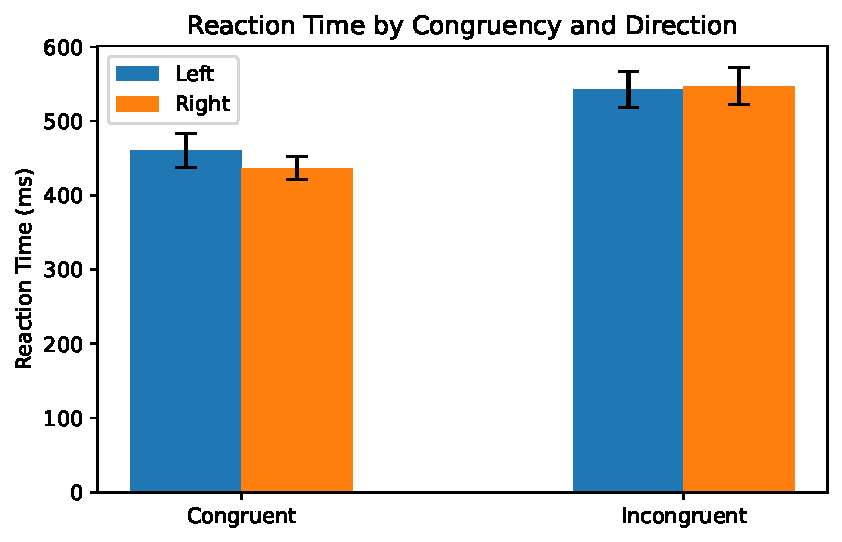
\includegraphics[keepaspectratio]{390JournalManuscript_files/figure-pdf/fig-rt-output-1.pdf}}

}

\caption{\label{fig-rt}Mean reaction time (ms) by congruency and
direction. Error bars represent ±1 SEM.}

\end{figure}%

\subsection{Accuracy}\label{accuracy}

Accuracy was higher for congruent trials (M = .97) than for incongruent
trials (M = .81) across both directions. A one-way repeated measures
ANOVA revealed a significant main effect of congruency on accuracy (F(1,
15) = 10.70, p = .005), with higher accuracy on congruent trials. A 2 x
2 repeated measures ANOVA revealed a significant main effect of
congruency on accuracy (F(1, 14) = 8.60, p = .011). There was no
significant main effect of direction (F(1, 14) = 0.52, p = .484) and no
significant interaction between congruency and direction (F(1, 14) =
0.19, p = .673). The results for the reaction time of congruent trials
compared to the incongruent trials are depicted in Figure~\ref{fig-acc}.

\begin{figure}[H]

\centering{

\pandocbounded{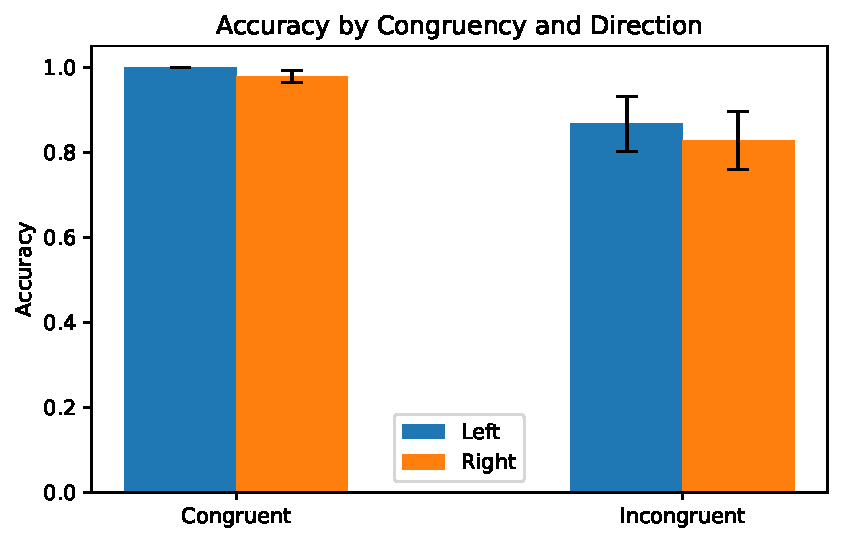
\includegraphics[keepaspectratio]{390JournalManuscript_files/figure-pdf/fig-acc-output-1.pdf}}

}

\caption{\label{fig-acc}Mean accuracy by congruency and direction. Error
bars represent ±1 SEM.}

\end{figure}%

\section{Discussion}\label{discussion}

\section{Conclusion}\label{conclusion}

Consistent with theories of selective attention and cognitive control,
the results of the present study provide clear support for the flanker
interference effect \citep{stoffels1988}. Specifically, participants
showed both slower response times and lower accuracy on incongruent
trials, indicating that flanker stimuli were automatically processed
even when they were task-irrelevant. This suggests that participants
were unable to fully suppress distracting information, highlighting the
limits of cognitive control under conditions of response conflict.

Also important to note is that the main effect of direction (left
vs.~right) was not significant, nor was the interaction between
direction and congruency, indicating that distractor congruency was the
primary driver of performance differences. This helps to strengthen the
interpretation that the observed flanker effects are due to interference
from competing stimuli rather than simple response biases.

Limitations: The small sample size (N = 16) reduces statistical power
and limits the generalizability of the findings. Additionally, the use
of a restricted sample of University of Waterloo students limits
variability in age and educational background, making the results less
representative of the broader population. The study also included only
20 trials per participant, which may reduce the reliability and
stability of both reaction time and accuracy measures. + randomized
sequences

Future Directions: Future research should address these limitations by
increasing sample size, diversifying participant demographics, and
including a greater number of trials to improve measurement reliability.
In addition, exploring individual differences in cognitive control
across populations could provide deeper insight into how interference
effects vary across contexts.

Overall, despite its limitations, this study successfully replicates a
well-established cognitive effect and demonstrates the robustness of the
flanker paradigm as a tool for studying attention and response conflict.


\renewcommand\refname{References}
\bibliography{bibliography.bib}



\end{document}
